\pagebreak
\section{Incomplete Tiles}
\label{sec:incomplete_tiles}

Optimal performance for tiled loops is achieved when the loop iteration count is a multiple of the tile size.
When this condition does not exist, the implementation is free to execute the partial loops in a manner that
optimizes performance, while preserving the specified order of iterations in the complete-tile loops.

Figure~\ref{fig:2d_tiling} shows an example of a 2-by-2 tiling for a 5-by-5 iteration space.
There are nine resulting tiles. Four are \emph{complete} 2-by-2 tiles, and the
remaining five tiles are \plc{partial} tiles.

\begin{figure}[H]
\begin{subfigure}[b]{.5\textwidth}
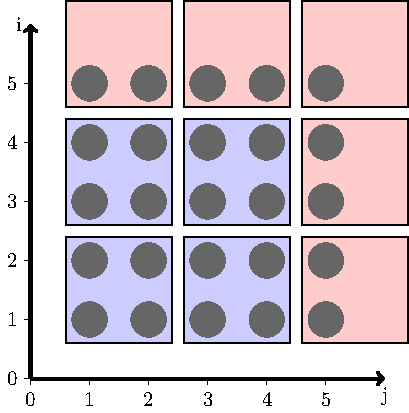
\includegraphics[width=0.8\textwidth]{figs/tile-2d_tiling}
\centering
\caption{2-dimensional tiling with partial tiles}\label{fig:2d_tiling}
\end{subfigure}%
\begin{subfigure}[b]{.5\textwidth}
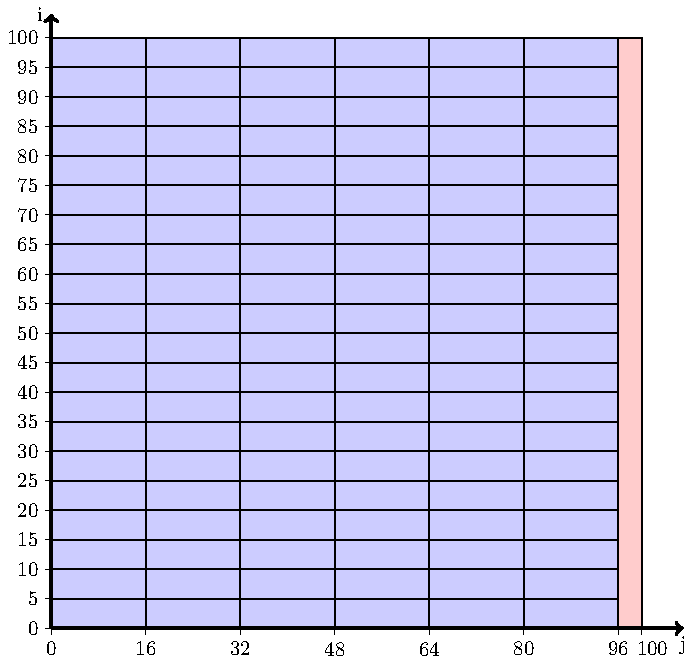
\includegraphics[width=0.85\textwidth]{figs/tile-Example_tile2}
\vspace*{2mm}
\centering
\caption{Partial tiles of Example \emph{partial\_tile.1}}\label{fig:Example_tile2}
\end{subfigure}
\caption{Tiling illustrations}
\end{figure}

In the following example, function \plc{func1} uses the \code{tile} construct
with a \code{sizes(4,16)} tiling clause.  Because the second tile dimension of
16 does not evenly divide into the iteration count of the j-loop, the
iterations corresponding to the remainder for the j-loop correspond to partial
tiles as shown in Figure~\ref{fig:Example_tile2}. Each remaining function
illustrates a code implementation that a compiler may generate to implement the
\code{tile} construct in \plc{func1}.

%Iterations with the tiles can be executed in a any order, ignoring partial tile boundaries.
% Deepak: I don't think this first sentence is true for iterations in a partial tile.
% Only the product order will be maintained for such iterations.
The order of tile execution relative to other tiles can be changed, but execution order of 
iterations within the same tile must be preserved.
Implementations must ensure that dependencies that are valid with any tile size need
to be preserved (including tile size of 1 and tiles as large as the iteration space).

Functions \plc{func2} through \plc{func6} are valid implementations of \plc{func1}.
In \splc{func2} the unrolling is illustrated as a pair of nested loops with a simple
adjustment in the size of the final iteration block in the \splc{j2} iteration space
for the partial tile.

Performance of the implementation depends on the hardware architecture, the instruction set and compiler optimization goals.
Functions \plc{func3}, \plc{func4}, and  \plc{func5} have the advantage that
the innermost loop for the complete tile is a constant size and can be replaced with SIMD instructions.
If the target platform has masked SIMD instructions with no overhead, then avoiding the construction of a
remainder loop, as in \plc{func5}, might be the best option.
Another option is to use a remainder loop without tiling, as shown in \plc{func6}, to reduce control-flow overhead.

\cexample[5.1]{partial_tile}{1}
\ffreeexample[5.1]{partial_tile}{1}


In the following example, function \plc{func7} tiles nested loops with a size of (4,16),
resulting in partial tiles that cover the last 4 iterations of the j-loop, as
in the previous example.  However, the outer loop is parallelized with a
\code{parallel} worksharing-loop construct.

Functions \plc{func8} and \plc{func9} illustrate two implementations of the tiling
with \code{parallel} and worksharing-loop directives.  Function \plc{func8} uses a single outer loop, with a \plc{min} function
to accommodate the partial tiles. Function \plc{func9}
uses two sets of nested loops, the first iterates over the complete tiles and the
second covers iterations from the partial tiles. When fissioning loops that
are in a \code{parallel} worksharing-loop region, each iteration of each workshared loop
must be executed on the same thread as in an un-fissioned loop.  The \code{schedule(static)} clause in \plc{func7}
forces the implementation to use static scheduling and allows the fission in function \plc{func8}.
When dynamic scheduling is prescribed, fissioning is not allowed.  When no scheduling is specified,
the compiler implementation will select a scheduling \plc{kind} and adhere to its restrictions.

\cexample[5.1]{partial_tile}{2}
\ffreeexample[5.1]{partial_tile}{2}
